
\begin{figure*}[ht]
% \label{fix:exp-results}
  \centering

  \begin{subfigure}[b]{0.45\textwidth}
    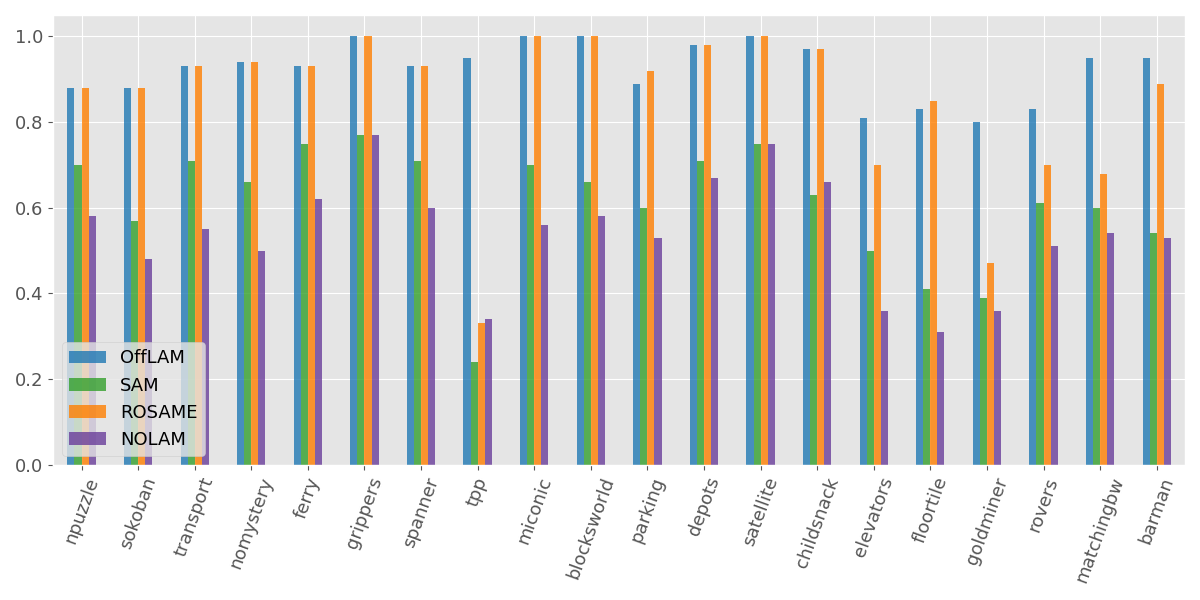
\includegraphics[width=\textwidth]{figures/10_traces/barplots/syn_precision.png}
    \caption{Syntactic precision}
    \label{fig:syn-precision}
  \end{subfigure}
  % \hfill
  \begin{subfigure}[b]{0.45\textwidth}
    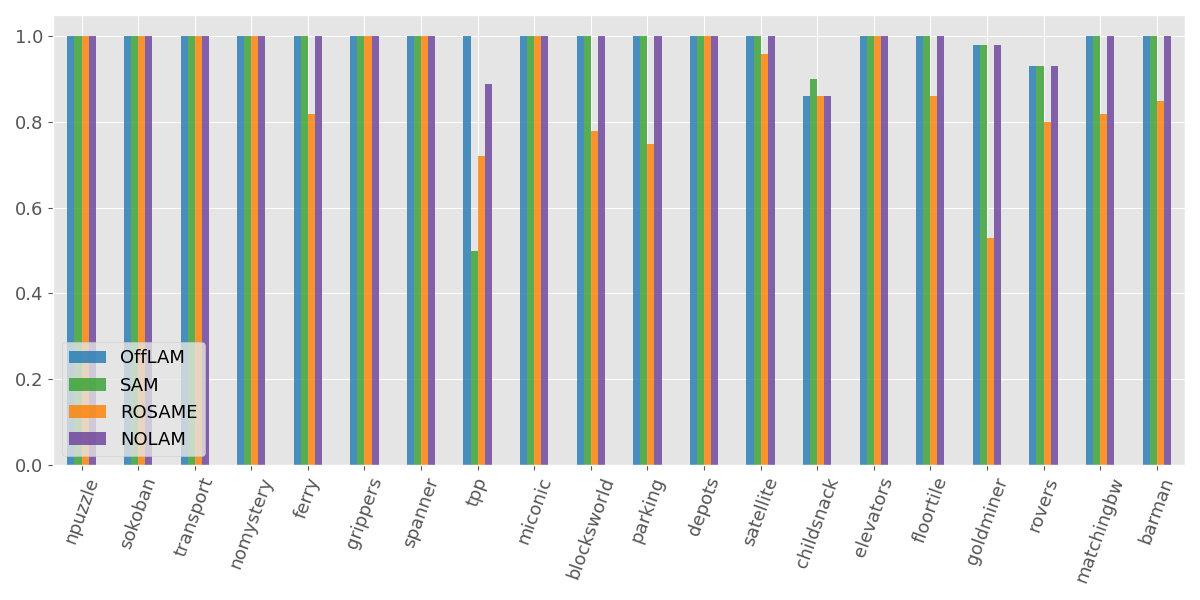
\includegraphics[width=\textwidth]{figures/10_traces/barplots/syn_recall.png}
    \caption{Syntactic recall}
  \end{subfigure}

  \vspace{1em}

  \begin{subfigure}[b]{0.45\textwidth}
    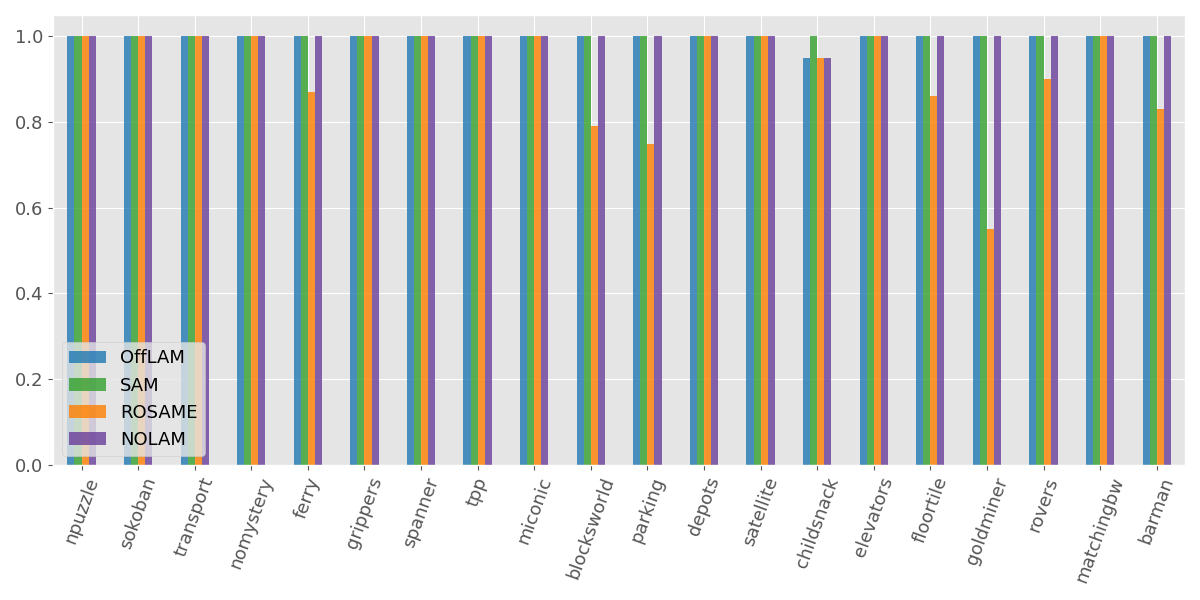
\includegraphics[width=\textwidth]{figures/10_traces/barplots/app_precision.png}
    \caption{Applicability precision}
  \end{subfigure}
  % \hfill
  \begin{subfigure}[b]{0.45\textwidth}
    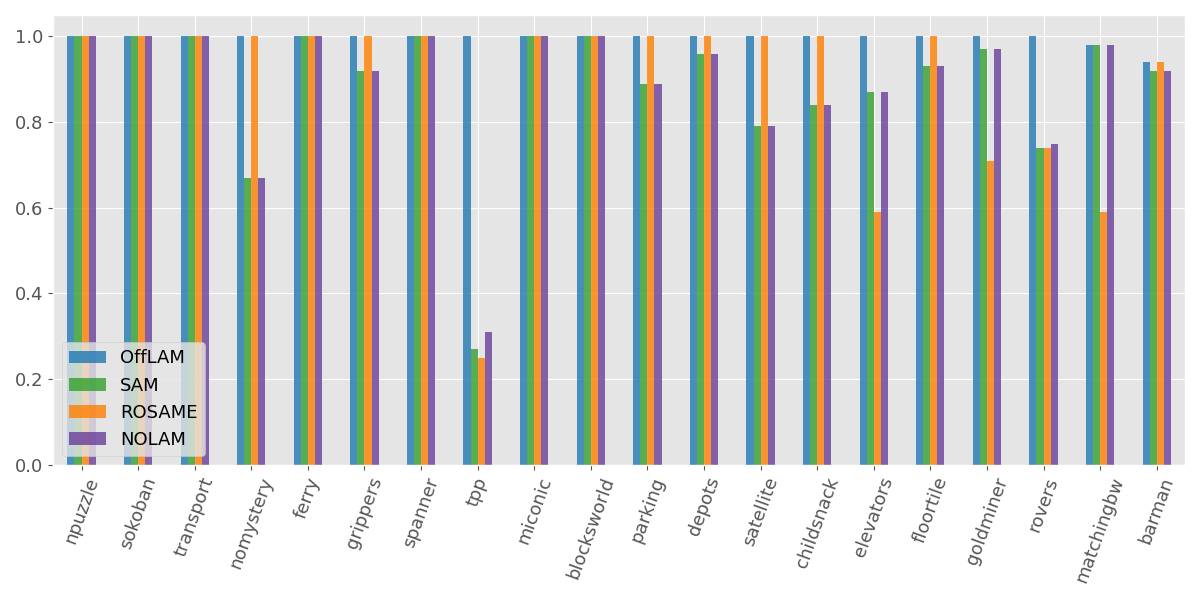
\includegraphics[width=\textwidth]{figures/10_traces/barplots/app_recall.png}
    \caption{Applicability recall}
  \end{subfigure}

  \vspace{1em}

  \begin{subfigure}[b]{0.45\textwidth}
    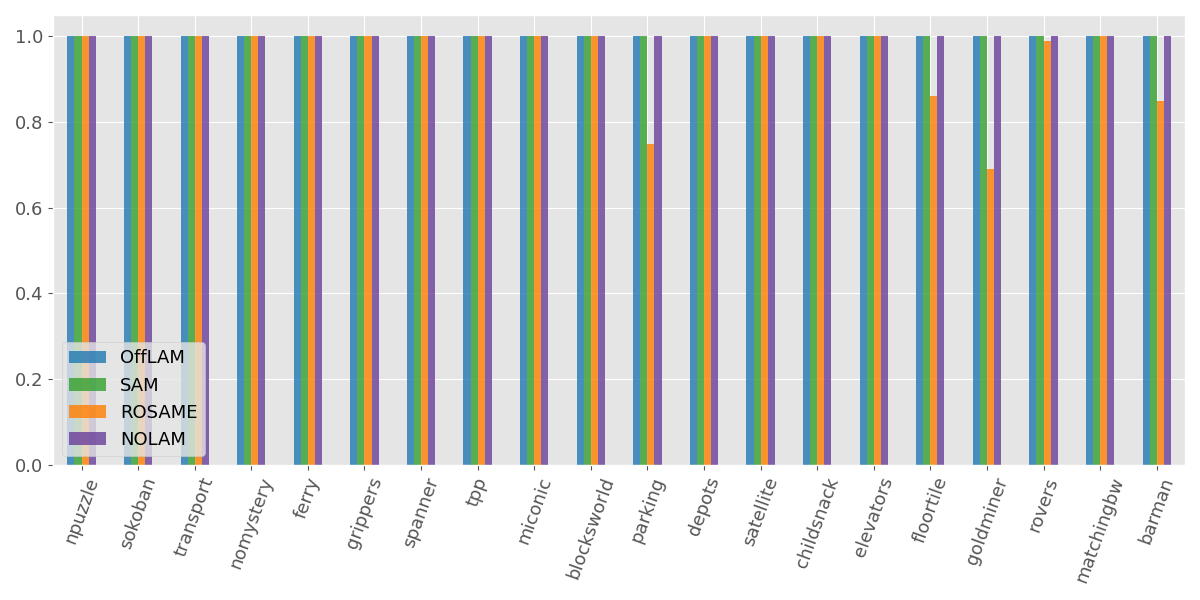
\includegraphics[width=\textwidth]{figures/10_traces/barplots/predeffs_precision.png}
    \caption{Predicted effects precision}
  \end{subfigure}
  % \hfill
  \begin{subfigure}[b]{0.45\textwidth}
    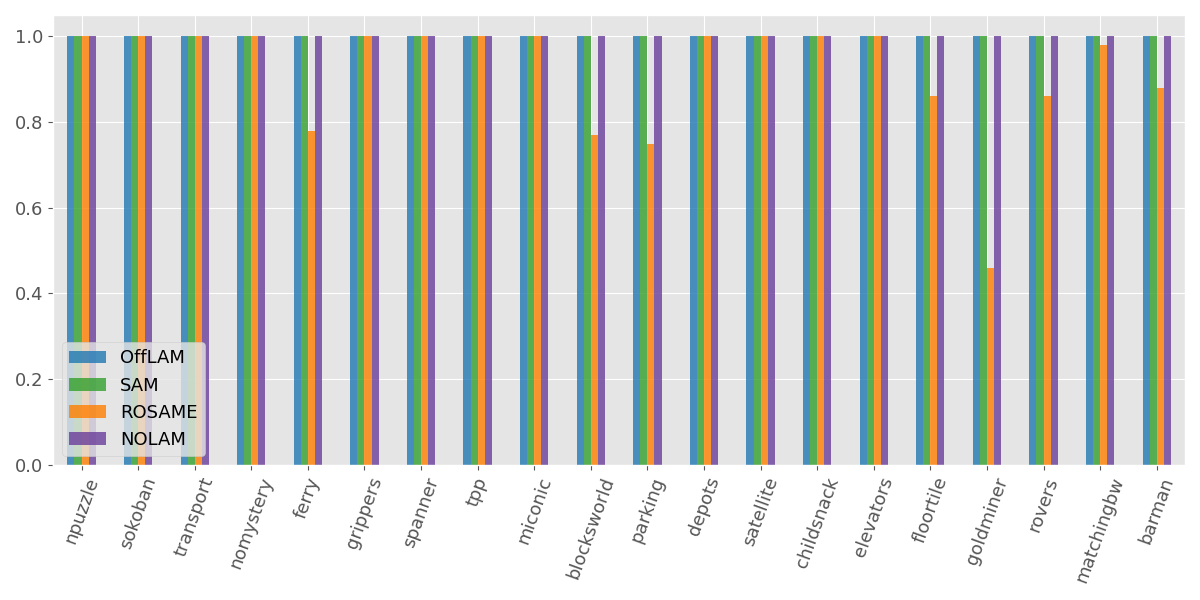
\includegraphics[width=\textwidth]{figures/10_traces/barplots/predeffs_recall.png}
    \caption{Predicted effects recall}
  \end{subfigure}

  \vspace{1em}

  \begin{subfigure}[b]{0.45\textwidth}
    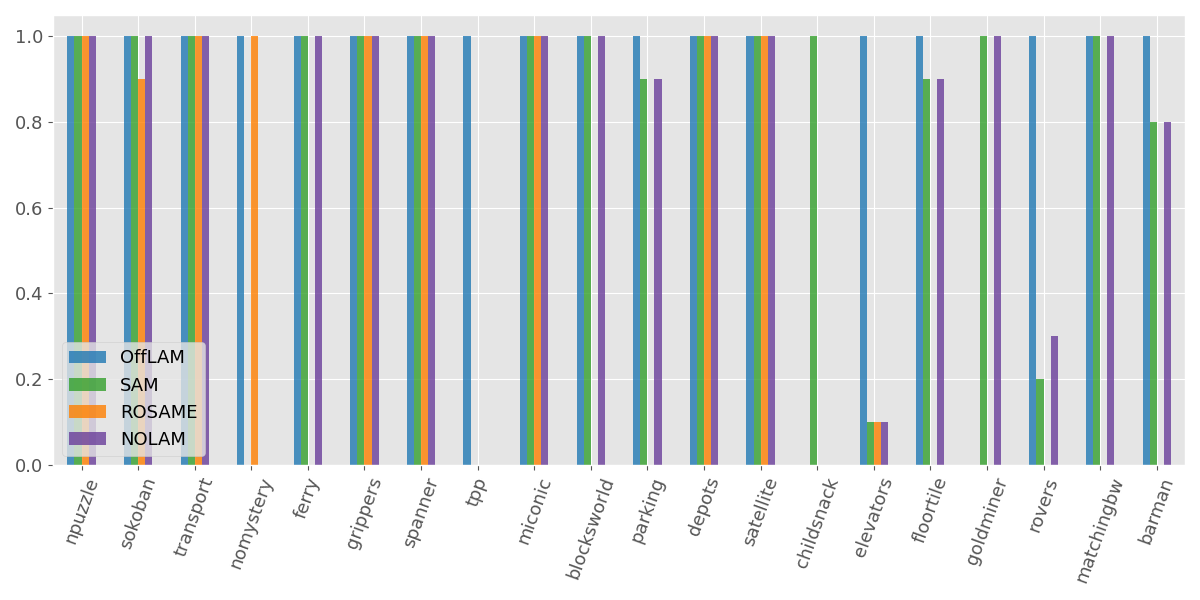
\includegraphics[width=\textwidth]{figures/10_traces/barplots/solving.png}
    \caption{Problem solving ratio}
    \label{fig:solving-ratio}
  \end{subfigure}
  % \hfill
  \begin{subfigure}[b]{0.45\textwidth}
    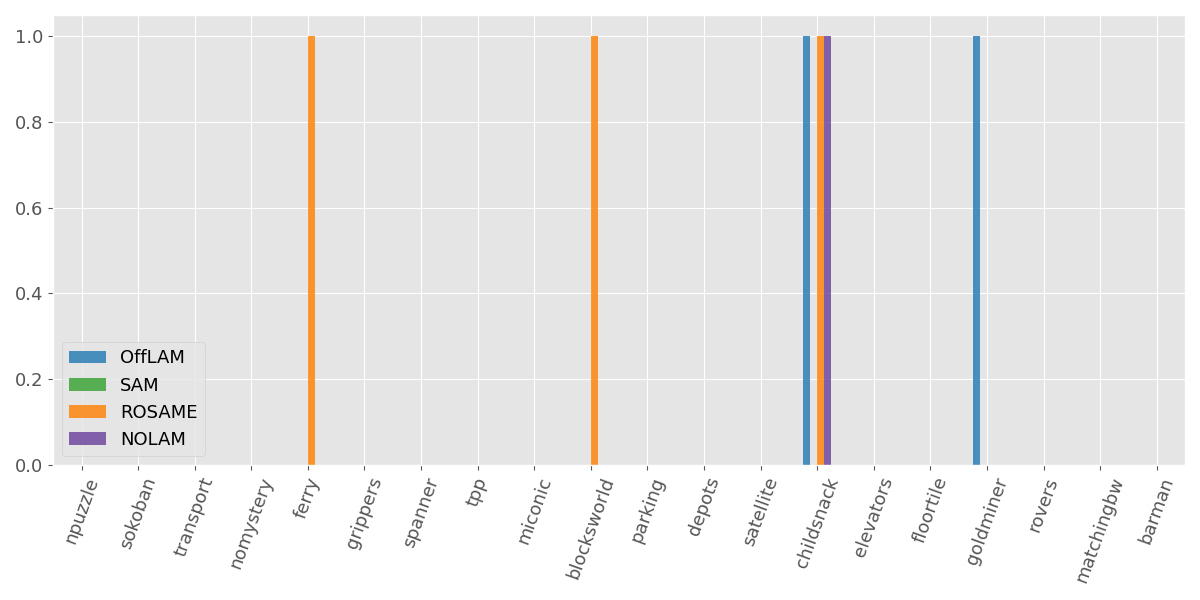
\includegraphics[width=\textwidth]{figures/10_traces/barplots/false_plans.png}
    \caption{False plans ratio}
    \label{fig:false-positive-plans}
  \end{subfigure}

  % \caption{Overall caption for the 6 images.}
  % \caption{Evaluation metrics when learning from a training set $\Ttrain$ with $10$ traces for every domain.}
\caption{Evaluation metric values for the models learned by \sam, \offlam, \nolam in every benchmark domain. The training set $\Ttrain$ includes $10$ trajectories for every domain.}
  % \label{fig:exp}
\end{figure*} 